
\graphicspath{ {SectionTheSimulationModule/Images/} }

\section{The Simulation Module}
\label{sec:the_simulation_module}

The Simulation Module implements one of the most fundamental tasks in the SML World, the Simulation of vehicles. It is, however, not limited to the simulation of the vehicle in itself, but also to the simulation of sensors that might be equipped in said vehicles.

In this the Simulation Module structure will be explained, as well as the simulation models used for the vehicles and for the vehicle sensors.

\subsection{The Simulation Module Class}

Remembering from the explanation given in \ref{subsubsec:simulation_module} (and additionally from figure \ref{fig:sml_world_structure_3}) we know that the Simulation Module will be running in an individual thread of execution in parallel with the SML World. It is however a part of the SML World, and it needs, by design, to interact with it.

The SimulationModule class, which implements the Simulator Module is defined in the file \texttt{SimulatorModule.py}. This class will have acess to the SML World, and it will interact heavily, reading and modifying, the vehicles stored in the Vehicles Dictionary.

\subsubsection{Constructor}

The constructor takes as arguments the SML World instance, and the desired simulation rate.

The SML World instance allows the Simulation Module class to have access to the SML World and its Vehicles Dictionary.

The second argument of the constructor, the desired simulation rate, defines the rate at which we wish the vehicles states and sensor readings to be updated (simulated). The Module will try to keep this rate as best as it can, however if it cannot keep up with this rate (due to low processing power for example), it will output warning messages to the terminal, letting the user know of this fact.

One can always reduce the desired rate of simulation in order to make sure that the Simulation Module can run at the desired rate. However the simulation quality decreases with the decrease of the simulation rate. By default the simulation rate is set to $50 Hz$.

The last step of the class constructor is creating the parallel thread of execution which will run the main loop.

\subsubsection{Main Loop}

The Main Loop of the class is defined in \texttt{thread\_loop}, and it is a fixed (given that there is enough processing power) rate loop that runs in parallel thread of execution while the SML World is running. This loop is responsible for calling the \texttt{simulate\_vehicles} and \texttt{simulate\_sensor\_readings} methods of the class.

\subsubsection{Vehicle Simulation}

The Vehicle Simulation is implemented by the \texttt{simulate\_vehicles} method, which will simply iterate over all the vehicles present in SML World's Vehicles Dictionary and update their states according to the simulation model used. The simulation model is defined by the Vehicle's Class method \texttt{vehicle\_state\_update}, and as such it is the task of the Vehicle Class to define the simulation model to be used. More details on the possible simulation models to use are provided in \ref{subsec:vehicle_models}.

The \texttt{simulate\_vehicles} method takes as argument \texttt{time\_to\_simulate} which corresponds to the amount, in seconds, of time that we wish to simulate. If the current vehicle states in the SML World correspond to time $t$, then the new updates states of said vehicles will correspond to time $t+\texttt{time\_to\_simulate}$.

The argument \texttt{time\_to\_simulate} is computed by the Main Loop (\texttt{thread\_loop}) and it will correspond to the time elapsed since the last call to \texttt{simulate\_vehicles} was made. This guarantees that even in situations where the desired simulation rate cannot be achieved, the simulation will compensate for it, and keep the vehicle states evolving in real time by simply simulate for a longer period of time. The inherent downside is that the simulation will inevitably lose quality. 


\subsubsection{Sensor Simulation}

The task of simulating the readings provided from the vehicle sensors is left to the \texttt{simulate\_sensor\_readings} method. Similarly to the \texttt{simulate\_vehicles} method, it will iterate over the vehicles present in the Bodies Dictionary, however instead of updating (altering) the vehicles' states it will change the vehicles' sensor readings. It does so by calling Vehicle's method \texttt{set\_sensor\_readings}.

This function does not have input arguments, but relies on the Vehicle Class' attributes to know which sensors to simulate. The boolean attributes \texttt{radar\_mode}, \texttt{velodyne\_mode} define if a Vehicle is equipped with Radar and/or Velodyne sensors, respectively. There is also the possibility to simulate a perfect sensor that is aware of every other vehicle in the SML World, and it can be turned on through the attribute \texttt{omniscient\_mode}. The implementation details of each sensor are given in \ref{subsec:sensor_models}.

\subsection{Vehicle Models}
\label{subsec:vehicle_models}

The vehicle models define how the vehicle states will evolve when being simulated. They can be made arbitrarily complex, in order to achieve realistic behaviour, however such models might be computationally expensive and slow. The choosing of an appropriate vehicle model is then a trade-off between realistic behaviour and computational efficiency. The current model used for the \texttt{smartvehicle.py} Vehicle Class is the Acceleration based Unicycle Model explained in \ref{subsubsec:acceleration_based_unicycle_model}.

\subsubsection{Kinematic Unicycle Model}
\label{subsubsec:kinematic_unicycle_model}

One of the simplest models to simulate a car movement is the kinematic model for a simple car with the position, $(x,y)$, and orientation, $\theta$, states. Said car has as commands a steering angle, $\phi$ and a linear velocity $v$.

Knowing the current state and command inputs, we can compute the derivatives of the state as 

\[
\label{eq:kinematic_car_model}
\begin{array}{rcl}
\dot{x} & = & v \cos{\theta} \\
\dot{y} & = & v \sin{\theta} \\
\dot{\theta} & = & ( \nicefrac{v}{L} ) \tan{\phi} 
\end{array}
\]

Parameter $L$ corresponds to the distance between the front and rear axles of the car. Knowing the derivatives of the state we can compute the next state, $\Delta t$ seconds after the current state using the approximation

\[
\begin{array}{rcl} 
x_{t+\Delta t} & = & x + \dot{x} \times \Delta t \\
y_{t+\Delta t} & = & y + \dot{y} \times \Delta t \\
\theta_{t+\Delta t} & = & \theta + \dot{\theta} \times \Delta t \\
\end{array}
\]

Of course the bigger the $\Delta t$, the rougher the estimation. That is why one should have an high simulation rate, as $\Delta t$ is the inverse of the simulation rate $\Delta t = \nicefrac{1}{\texttt{simulation\_rate}}$.

\subsubsection{Acceleration based Unicycle Model}
\label{subsubsec:acceleration_based_unicycle_model}

The acceleration based unicycle model builds upon the kinematic unicycle model described before, however it now adds assumes that the linear velocity of the car is follows an acceleration model equation.

To implement such a model, the vehicle state has to now include the velocity states $(\dot{x},\dot{y})$, which are used to determine the instantaneous linear velocity $v=\sqrt{\dot{x}^2 + \dot{y}^2}$. Furthermore, instead of a velocity command input, we now have a throttle command input. The evolution of the $(x,y,\theta)$ states will still be described by equations \ref{eq:kinematic_car_model}, however the evolution of the linear car velocity $v$ is given by:

\[
\dot{v} = \frac{throttle - c\times v}{m}
\]

Where $throttle$ is the throttle produced by the car, $c$ is the air drag coefficient of the car, and $m$ its mass.

\subsection{Sensor Models}
\label{subsec:sensor_models}

Sensor models are used to determine what information a sensor can provide to a car given its current surroundings. The sensor models used here will assume that the sensor is capable of processing the information it gathers, and convert it to an understandable vehicle state given by $(x,y,\dot{x},\dot{y})$ and respective id.

The only difference between the sensors that will be described later is then related only to its region/area of sensing, that is, how far and wide can a sensor detect other vehicles.

By simulating the sensors in this way, we are jumping over one of the big problems of autonomous driving, the processing and understanding of data coming from sensors. This is not a problem however, since the current scope of the SML World does not focus on the area of Sensors and Data Fusion.

\subsubsection{Radar}

The Radar sensor will be able to detect vehicles that are in a cone shaped region situated in front of the ego vehicle. This region is defined by two attributes \texttt{radar\_angle} and \texttt{radar\_range}. The radar angle determines the field of sensing of radar, the larger it is the wider the sensing cone. The radar range in turn will determine how far can the radar sense, this can be thought of as the height of the cone. Figure \ref{fig:radar_sensing_area} shows the sensing cone of a vehicle's radar, and how these attributes shape the sensing area of the radar.

\begin{figure}[h!]
  \centering
    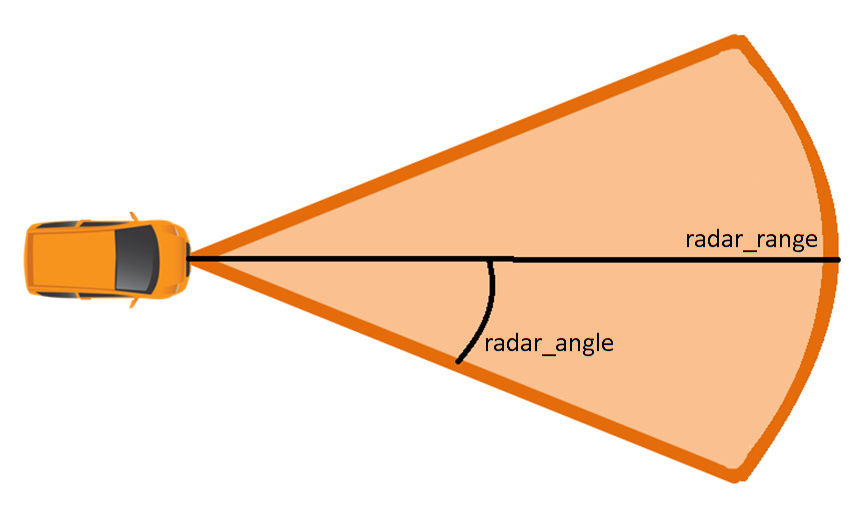
\includegraphics[width=0.9\textwidth]{radar_markings_quantities}
    \caption{Representation of the radar sensing area \label{fig:radar_sensing_area} }
\end{figure}

This sensor can be toggled on or off using the boolean attribute \texttt{radar\_mode}. The sensor provides readings for each vehicle in the sensing area in the form of $(id, x, y, \dot{x}, \dot{y})$.


\subsubsection{Velodyne}

The Velodyne sensor is a sensor used by KTH's Research Concept Vehicle which is able to sense objects in a 360 degree area. To completely define this sensor we just need to set the value of  \texttt{velodyne\_range} which determines the radius of the sensing circle of the Velodyne. Figure \ref{fig:velodyne_sensing_area} shows the sensing area of this sensor.

\begin{figure}[h!]
  \centering
    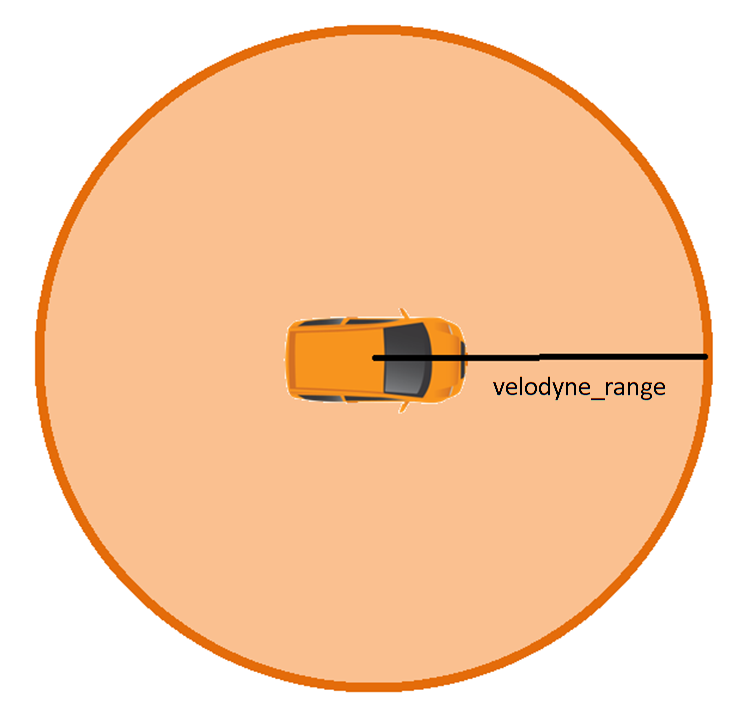
\includegraphics[width=0.75\textwidth]{velodyne_markings_quantities}
    \caption{Representation of the velodyne sensing area \label{fig:velodyne_sensing_area} }
\end{figure}

The Velodyne sensor can be toggled on or off using the boolean attribute \texttt{velodyne\_mode}. The sensor provides readings for each vehicle in the sensing area in the form of $(id, x, y, \dot{x}, \dot{y})$.

\subsubsection{Omniscience}

A perfect sensor can also be simulated by toggling the attribute \texttt{omniscient\_mode}. If activated this sensor will get the readings of every vehicle present in the SML World, no matter how far they might be. The sensor will thus provide readings for all the vehicle in the SML World in the form of $(id, x, y, \dot{x}, \dot{y})$.


